
\section{System development task}\label{sec:task}

The system development task for this thesis is to complete the backend of Comordo's system. This includes the reader, input, output and parameter modules, the storage of purchase history and parameters and modules for parameter tuning. The other databases were provided, but some level of adaptation was needed. The recommender algorithms \textit{katz-eig} and \textit{link-analysis} were given and again some adaptation was needed. The admin interface and the remote API are outside the scope of this thesis.

\Figureref{fig:sysoverview} is the system sketch of Comordo's recommender system, as planned for at the start of this thesis.

\begin{figure}[h!]
  \centering
    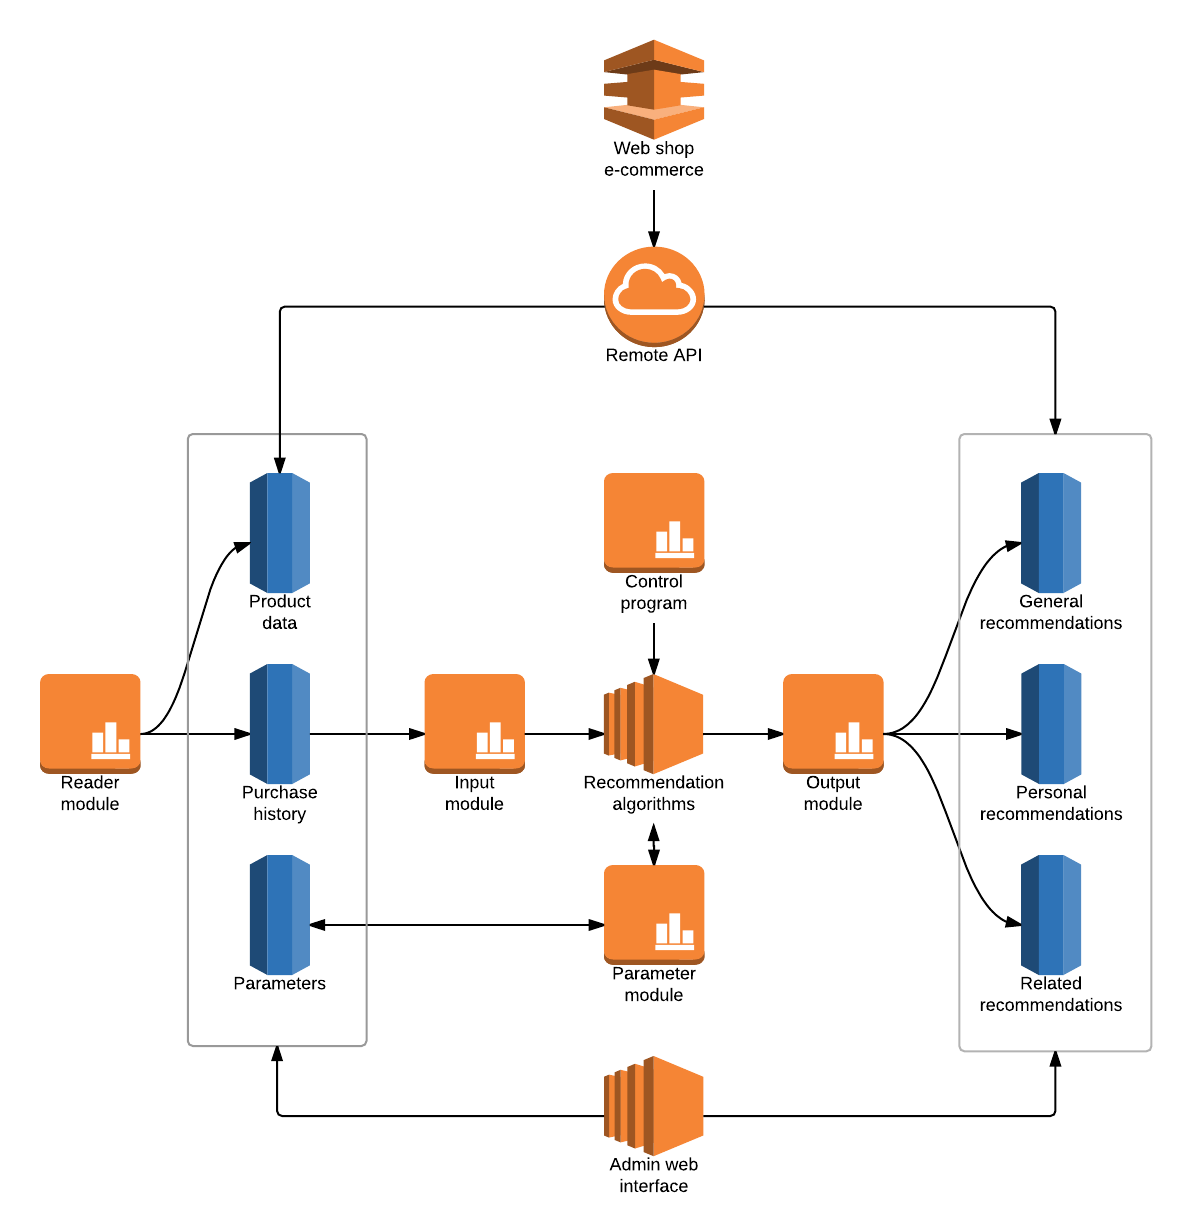
\includegraphics[width=0.9\textwidth]{fig/system_overview.png}
  \caption{Comordo's system sketch}
  \label{fig:sysoverview}
\end{figure}

\FloatBarrier

\begin{description}
    \item[Reader module] is responsible for reading data files provided by Comordo's clients.
    \item[Input module] provides the algorithms with transformed data.
    \item[Output module] populates the database with recommendations.
    \item[Control program] handles learning and optimization of the algorithms.
    \item[Parameter module] stores and adjusts parameters the algorithms use.
    \item[Remote API] is a REST based API, the endpoint for Comordo's clients.
    \item[Admin web interface] is a user friendly way for e-commerce clients to customize system settings and view recommendations.
\end{description}


\subsection{Use case}\label{sec:use}

This is a high level use case for how Comordo's recommender system will be used via the remote API and how recommendations will be produced for Comordo's clients.

\begin{enumerate}
    \item Purchase history and product data is provided by e-commerce clients and consumed by the recommender system.
    \item Load algorithms with purchase history and produce recommendations.
    \item Repopulate recommendation database with new recommendations.
    \item Final customers visit the e-commerce website and are given recommendations delivered to the website via Comordo's remote API.
\end{enumerate}

